% Preamble
\documentclass[14pt, aspectration=169]{beamer}
\usetheme{Copenhagen}
\usecolortheme{beaver}

\setbeamertemplate{navigation symbols}{}

% Packages
\usepackage{amsmath}
\usepackage{listings}
\usepackage{xcolor}
\usepackage{blkarray}
\usepackage{graphicx}

\definecolor{codegreen}{rgb}{0,0.6,0}
\definecolor{codegray}{rgb}{0.5,0.5,0.5}
\definecolor{codepurple}{rgb}{0.58,0,0.82}
\definecolor{backcolour}{rgb}{0.95,0.95,0.92}

\lstdefinestyle{mystyle}{
    backgroundcolor=\color{backcolour},
    commentstyle=\color{codegreen},
    keywordstyle=\color{magenta},
    numberstyle=\tiny\color{codegray},
    stringstyle=\color{codepurple},
    basicstyle=\ttfamily\footnotesize,
    breakatwhitespace=false,
    breaklines=true,
    captionpos=b,
    keepspaces=true,
    numbers=left,
    numbersep=5pt,
    showspaces=false,
    showstringspaces=false,
    showtabs=false,
    tabsize=4
}

\lstset{style=mystyle}

\title{Introduction to Advanced Python:\\Why is Python slow?}
\author{Kai Striega}
\date{\today}

% Document
\begin{document}

    \maketitle

    \begin{frame}{Before I start}
        \begin{block}{Here be dragons}<2->
            This talk introduces advanced topics, quickly.
            The content is designed to stretch your understanding and to challenge you.
        \end{block}
        \begin{block}{Questions}<3->
            I am happy to take questions during the talk, feel free to ask if something doesn't make sense.
        \end{block}
    \end{frame}

    \begin{frame}{What we're going to do today}
        \begin{itemize}
            \item<2-> Answer the question: Why is Python slow?
            \item<3-> Compare Python to C and assembly
            \item<4-> Introduce some of the key ideas in performance analysis
            \item<5-> Discuss when execution time matters\ldots and when it doesn't
        \end{itemize}
    \end{frame}

    \begin{frame}{Why C?}
        \begin{columns}
            \column{0.55\textwidth}
            \begin{itemize}
                \item C is \textit{very} fast
                \item Python is written in C
                \item Many Python extensions are written in C
            \end{itemize}
            \column{0.45\textwidth}
            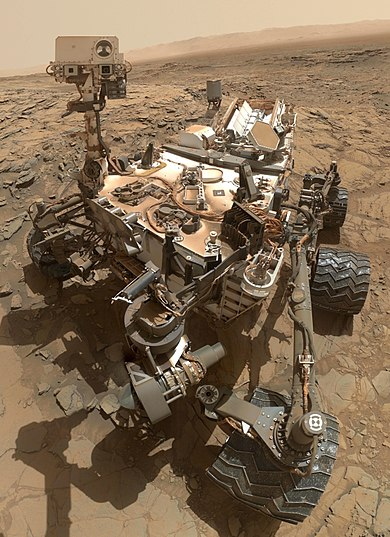
\includegraphics[scale=0.35]{static/images/390px-Curiosity_Self-Portrait_at_'Big_Sky'_Drilling_Site}
        \end{columns}
    \end{frame}
    \begin{frame}{Today's Example}
        \lstinputlisting[language=Python,label={lst:python}]{code/sum_of_first_n_numbers.py}
    \end{frame}

    \begin{frame}{Is Python slow?}
        \begin{itemize}
            \item[]<2-> \texttt{time python sum\_of\_first\_n\_numbers.py\newline}
            \item[]<3-> \texttt{total=18446744064889498501\newline
            real 5m56.581s\newline
            user 5m56.518s\newline
            sys 0m0.004s\newline}
        \end{itemize}
    \end{frame}

    \begin{frame}{Today's Example, but in C}
        \lstinputlisting[language=C,label={lst:C}]{code/sum_of_first_n_numbers.c}
    \end{frame}

    \begin{frame}{What about C?}
        \begin{itemize}
            \item[]<2-> \texttt{time bin/sum\_of\_first\_n\_numbers\_O3\newline}
            \item[]<3-> \texttt{total=18446744064889498501\newline
            real 0m0.000s\newline
            user 0m0.000s\newline
            sys 0m0.000s\newline}
        \end{itemize}
    \end{frame}

    \begin{frame}{Why?}
        \begin{itemize}
            \item \textit{0m0.000s} seems like a bug\ldots but it's not!
            \item C is a \textbf{compiled} langauge
            \item That means the compiler can perform optimizations before the code is run
        \end{itemize}
    \end{frame}

    \begin{frame}{Assembly}
        \begin{itemize}
            \item I'm about to show you a language called \textit{Assembly}
            \item Assembly corresponds to the CPU's machine instructions
            \item a.k.a. the instructions the CPU is executing
            \item Assembly is specific to your CPU architecture
        \end{itemize}

        \begin{alertblock}{Assembly}<2->
            Assembly is a new topic that you (probably) won't have to know in depth.
            It is included here to analyse the code being run by C, but you won't have to remember the in and outs of
            assembly.
        \end{alertblock}
    \end{frame}

    \begin{frame}{What C does}
        \lstinputlisting[label={lst:asm-O3-no-arg}]{static/code/sum_clang_17_O3.asm}
    \end{frame}

    \begin{frame}{Today's Example, in C, with arguments}
        \lstinputlisting[language=C,label={lst:C-args}]{code/sum_of_first_n_numbers_arg.c}
    \end{frame}

    \begin{frame}{What about with an argument?}
        \begin{itemize}
            \item[]<2-> \texttt{time bin/sum\_of\_first\_n\_numbers\_arg\_O3\newline}
            \item[]<3-> \texttt{total=18446744064889498501\newline
            real 0m0.000s\newline
            user 0m0.000s\newline
            sys 0m0.000s\newline}
        \end{itemize}
    \end{frame}

    \begin{frame}{What C does (with an argument)}
        \lstinputlisting[label={lst:asm-O3-arg}]{static/code/sum_arg_clang_17_O3.asm}
    \end{frame}

    \begin{frame}{What has the compiler done for me lately?}
        \begin{itemize}
            \item There's an alternate way to calculate the sum of the first $n$ numbers
            \item $\frac{n(n + 1)}{2}$
            \item The compiler transformed the algorithm from one with linear runtime to constant runtime
        \end{itemize}
    \end{frame}

    \begin{frame}{What C does (without optimizations)}
        \lstinputlisting[label={lst:asm-O3-arg-O0}]{static/code/sum_arg_clang_17_O0.asm}
    \end{frame}

    \begin{frame}{What if we don't use optimizations?}
        \begin{itemize}
            \item[]<2-> \texttt{time bin/sum\_of\_first\_n\_numbers\_arg\_O0\newline}
            \item[]<3-> \texttt{total=18446744064889498501\newline
            real 0m2.020s\newline
            user 0m2.010s\newline
            sys 0m0.010s\newline}
        \end{itemize}
    \end{frame}

    \begin{frame}{What we've done so far}
        \begin{itemize}
            \item We've turned a 6-minute problem into a 2-second problem
            \item Just by changing language
            \item This speedup exists even without optimizations enabled
            \item What makes C so much faster than Python?
            \item[]<2->
            \begin{itemize}
                \item The Python interpreter
                \item Poor memory usage
            \end{itemize}
        \end{itemize}
    \end{frame}

    \begin{frame}{The Python Interpreter}
        \begin{itemize}
            \item We say that Python is an \textbf{interpreted} language
            \item Python has to \textbf{interpret} the provided \texttt{.py} file before it can be run
            \item Interpreting code is expensive - there are many steps to it, and it takes (a lot) time
            \item We cannot apply many types of optimizations
        \end{itemize}
    \end{frame}
\end{document}